%% appendix.tex
%%

%% ==============================
\Appendix
\label{ch:Appendix}
%% ==============================



\section{Technische Dokumentation über die Benutzung der Segmentierungstools der MITK-Workbench}

Als erstes muss in den DICOM Ordner der Ordner mit ungefähr 200 Elementen gefunden werden.

\begin{figure}[H] 
\centering 
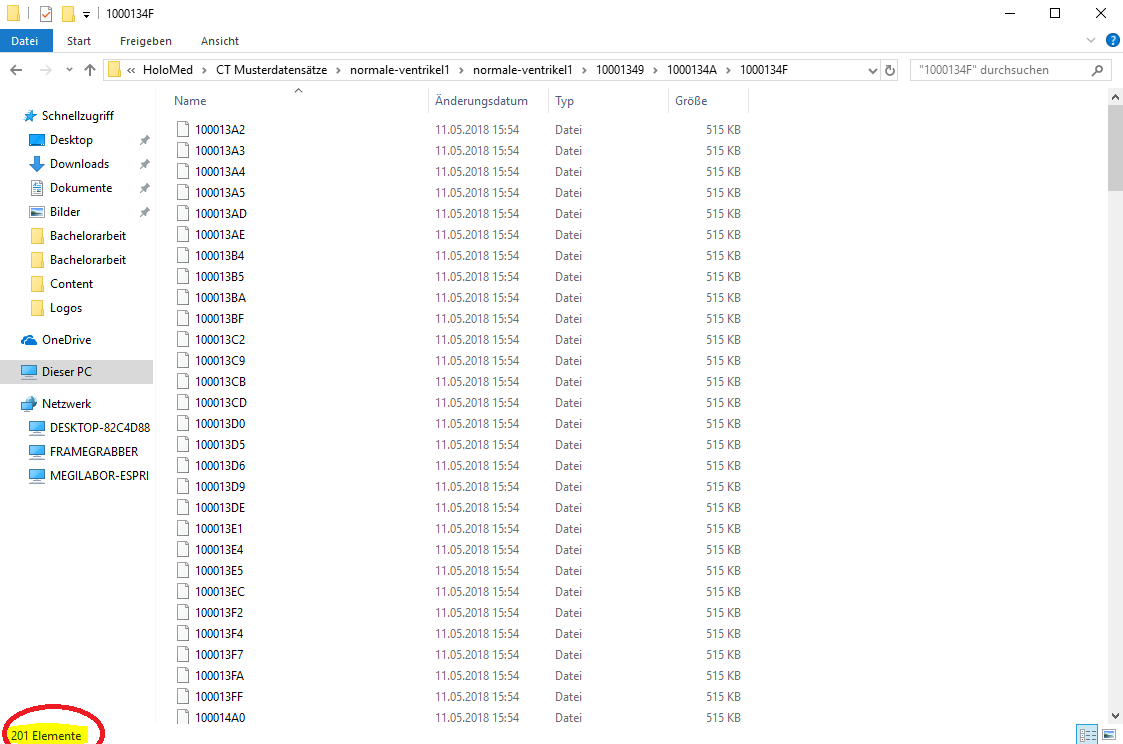
\includegraphics[width=0.7\textwidth]{Logos/MITK_Doku/1.PNG}
\caption{Ordner finden} 
\label{fig:eins} 
\end{figure}

Anschließend kann eine der Dateien des Ordners via drag and drop in den \textit{Data Manager} gezogen werden und das Fenster das erscheint bestätigt werden.
\newline
In der Mitte sind die verschiedenen Schnittbilder zu sehen, durch die mit dem Mausrad durchgegangen werden kann.
\newline
Die Zahlen von 1 bis 5 markieren verschiedenen Tools. Werden diese angeklickt, öffnet sich an der Seite oder unter den Schnittbildern das jeweilige Tool. Um ein Tool auf ein Volumen anzuweden, muss dieses immer im \textit{Data Manager} ausgewählt sein.
\newline
Mit dem Regler am rechten Rand der Schnittbilder kann die Darstellung der Grauwerte eingestellt werden.

\begin{figure}[H] 
\centering 
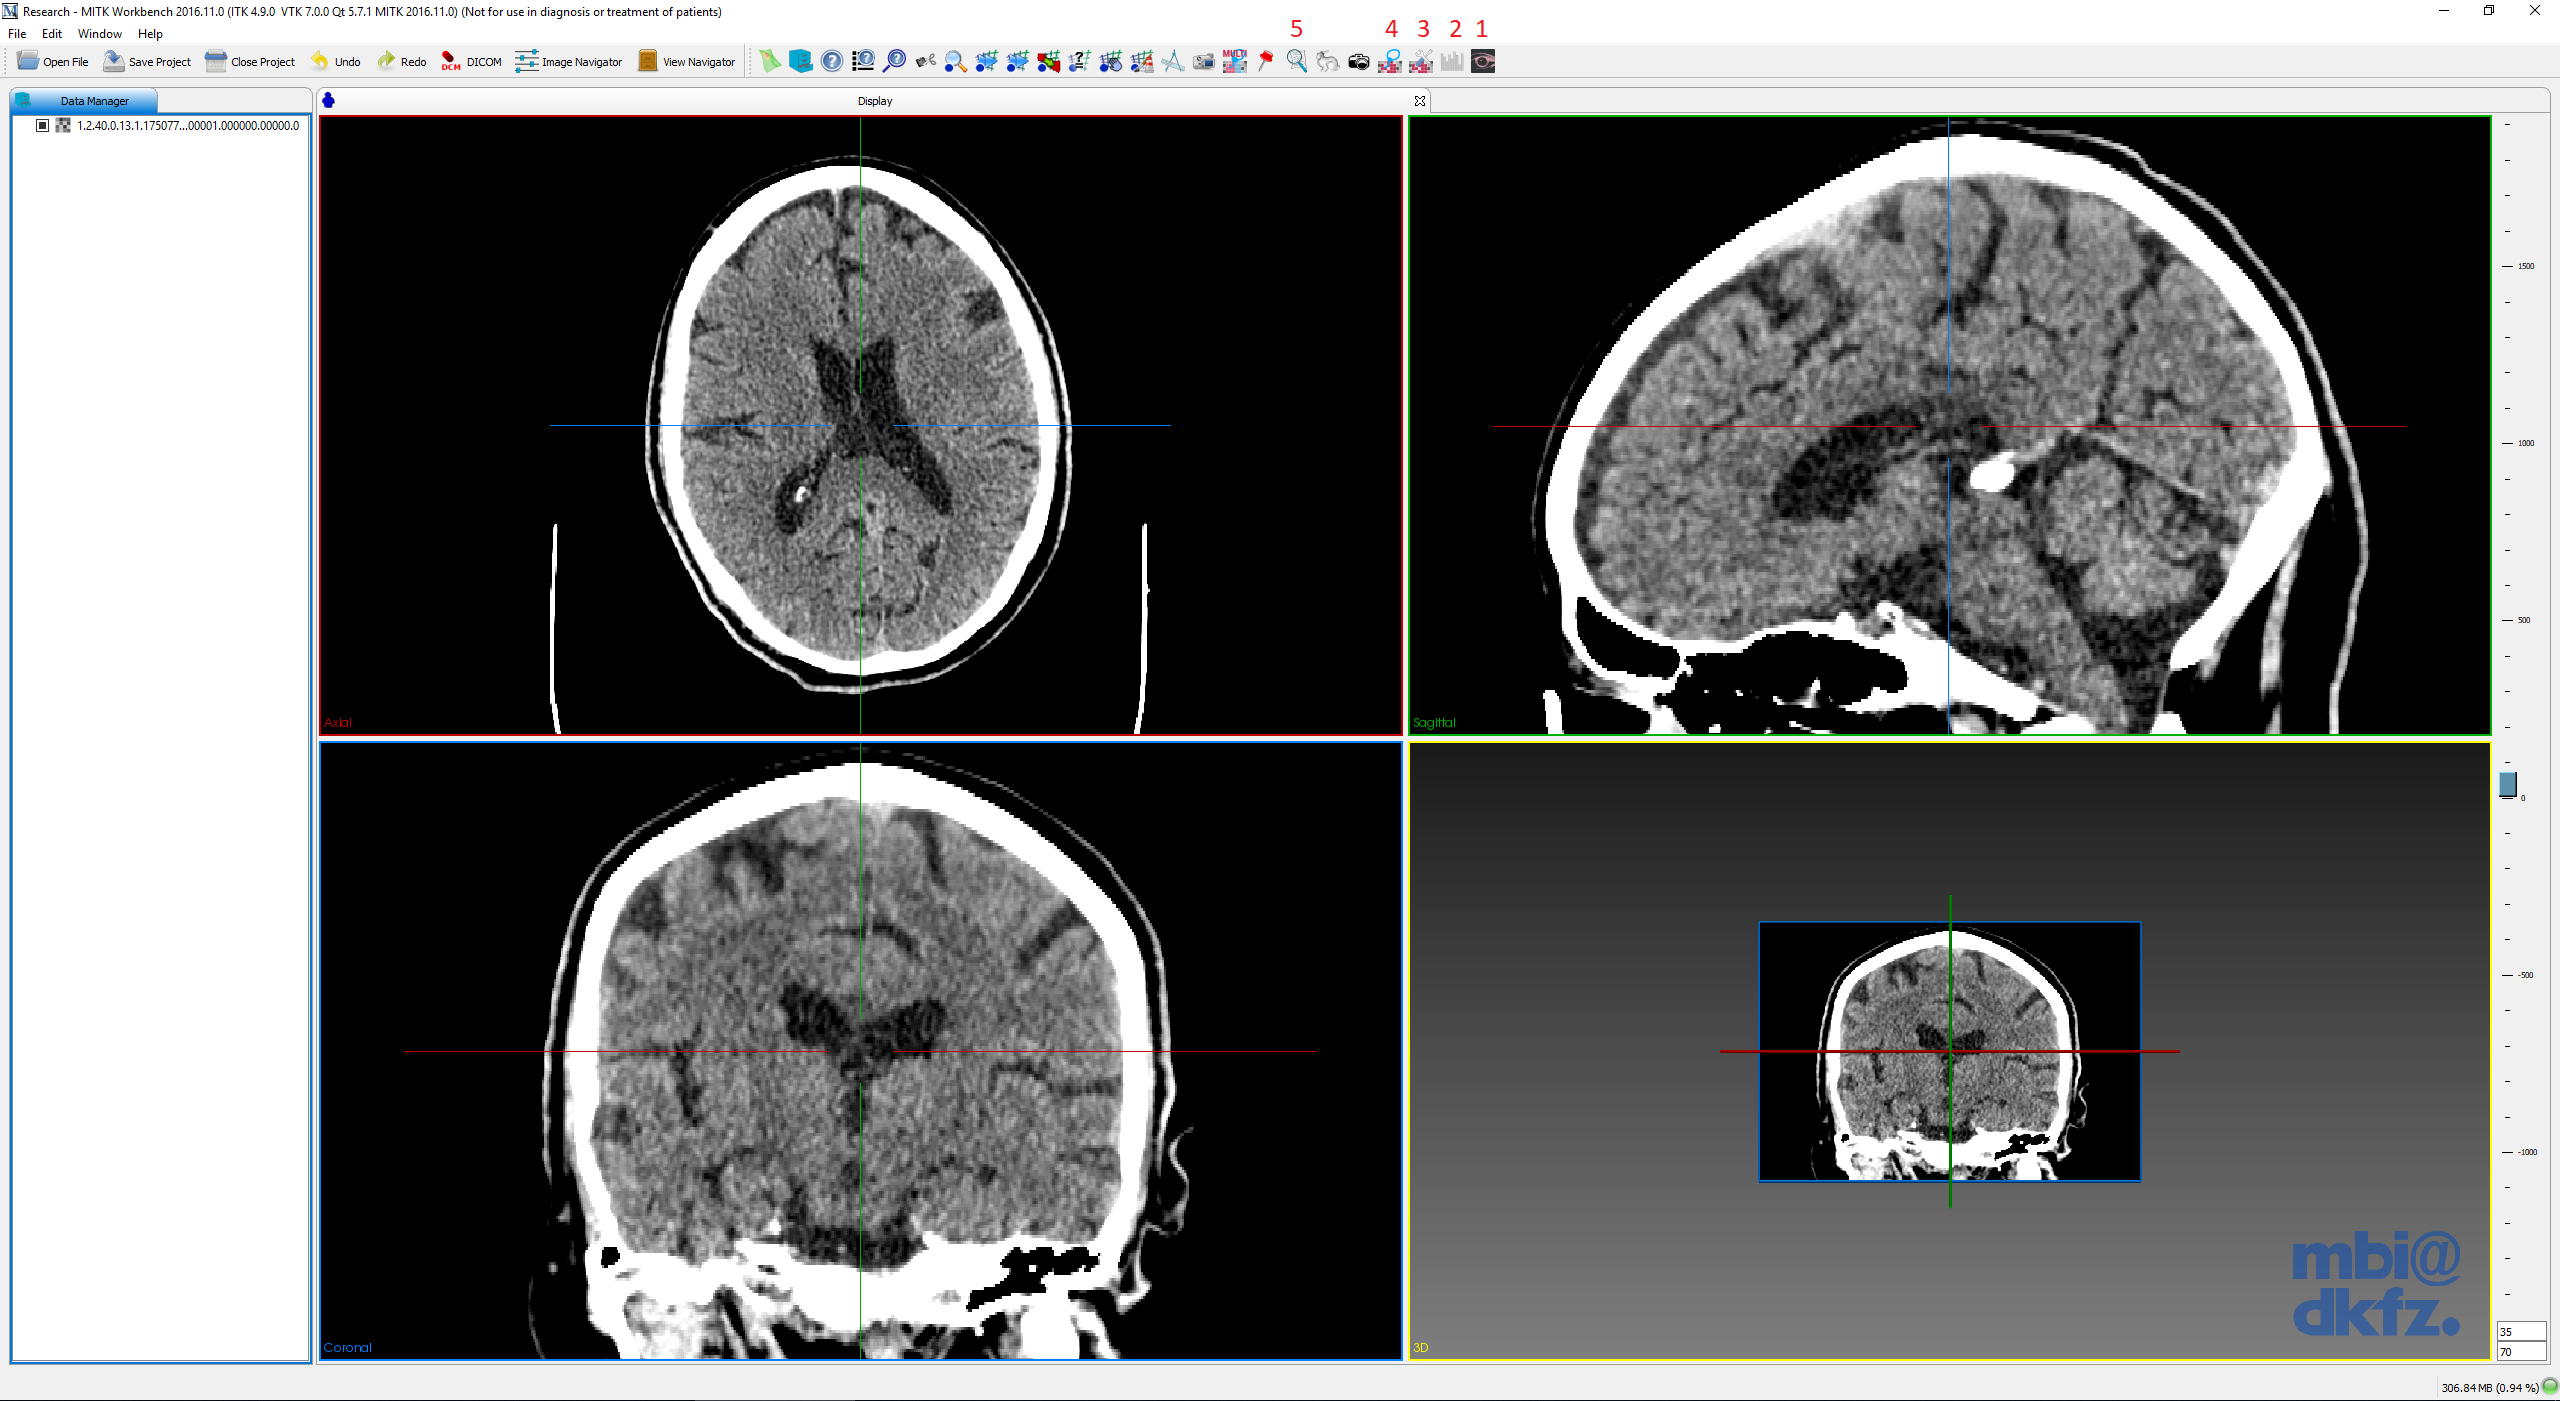
\includegraphics[width=\textwidth]{Logos/MITK_Doku/2.PNG}
\caption{Überblick über die Workbench} 
\label{fig:zwei} 
\end{figure}

Das Tool mit der Nummer 1 macht es möglich eine Transferfunktion zu definieren. Anhand der Intensitätswerte, den Punkten über dem Diagramm und dem Farbstrahl darunter kann die Transferfunktion angepasst werden. Ist der Haken bei \textit{Volumerendering} gesetzt, so wird die Visualisierung im Fenster links unten angezeigt.

\begin{figure}[H] 
\centering 
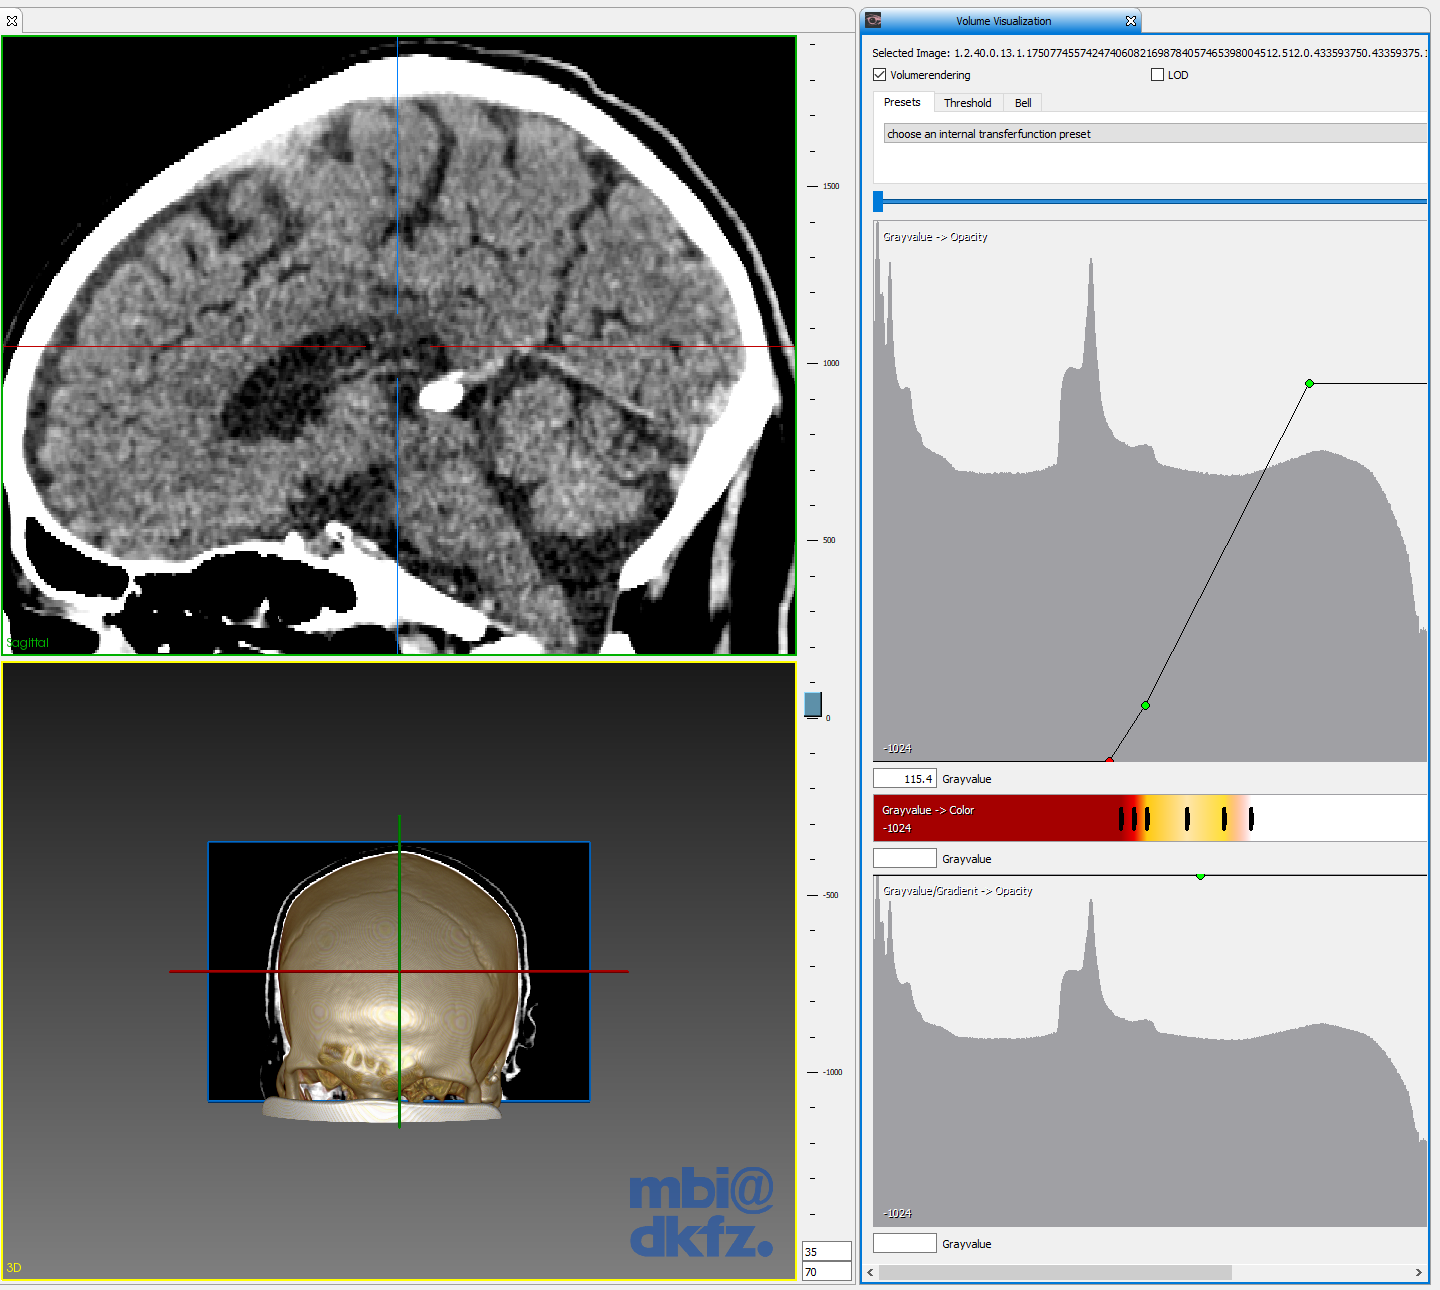
\includegraphics[width=0.7\textwidth]{Logos/MITK_Doku/3.PNG}
\caption{Transferfunktionstool der MITK-Workbench} 
\label{fig:drei} 
\end{figure}

Das Tool mit der Nummer 2 zeigt Statistiken zum Volumen an, wie zum Beispiel Verteilung der Intensitätswerte, der Median dieser etc.

\begin{figure}[H] 
\centering 
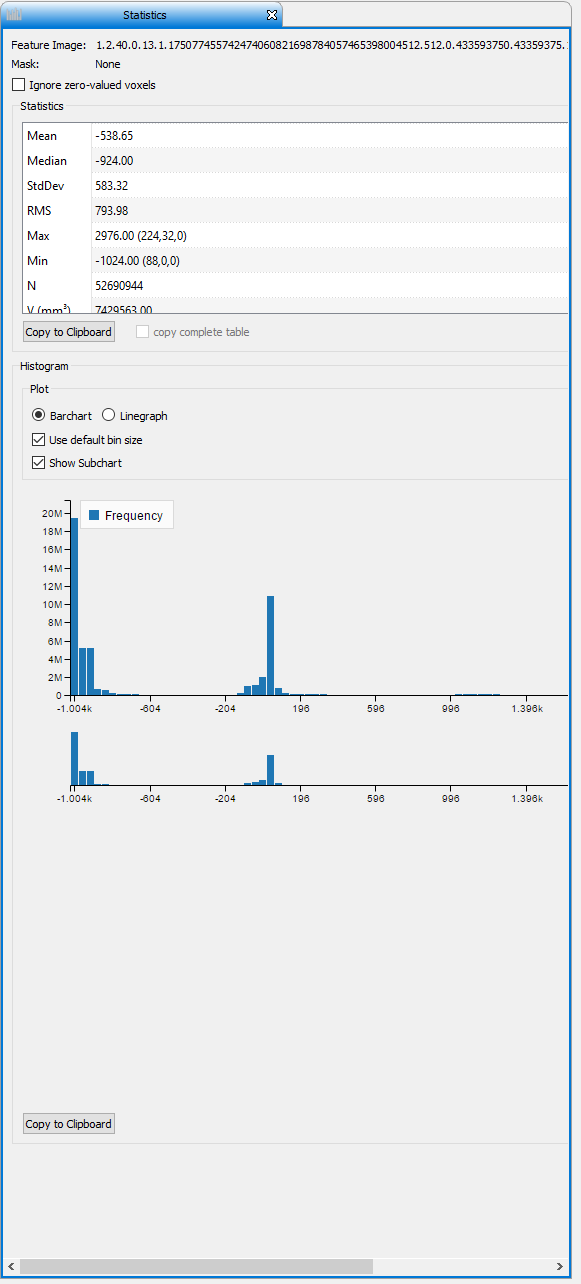
\includegraphics[width=0.4\textwidth]{Logos/MITK_Doku/4.PNG}
\caption{Statistiktool der MITK-Workbench} 
\label{fig:vier} 
\end{figure}

Das Tool Nummer 3  bietet verschiedene 2D und 3D Segmentierungstools an. Zunächst muss jedoch eine neue Segmentierung über den rot markierten Knopf erstellt werden.

\begin{figure}[H]
\centering 
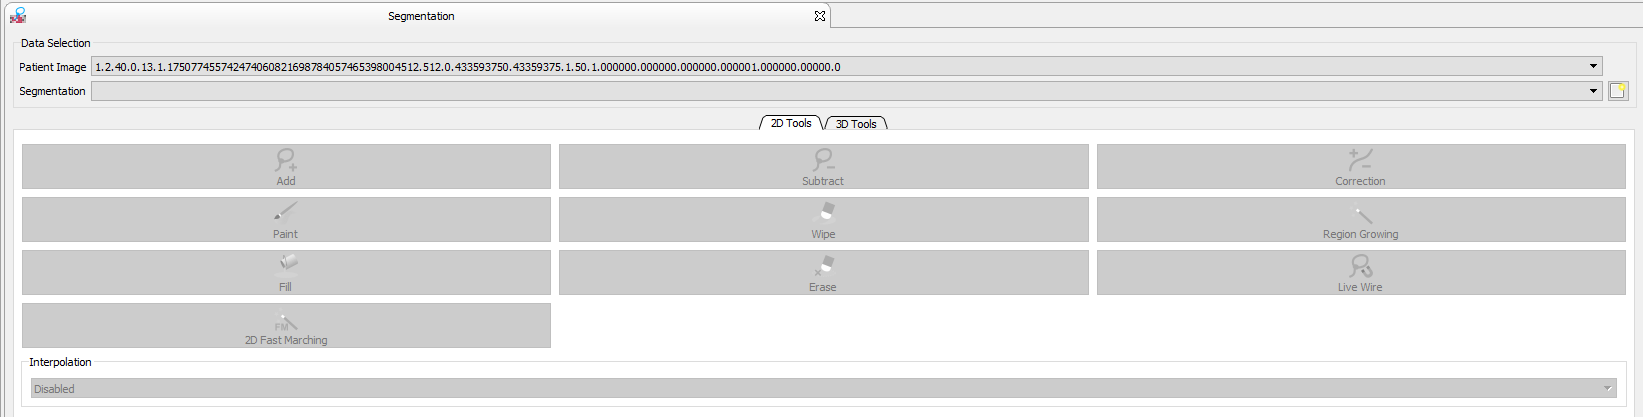
\includegraphics[width=0.7\textwidth]{Logos/MITK_Doku/5.PNG}
\caption{Segmentierungstools der MITK-Workbench} 
\label{fig:fuenf} 
\end{figure}

Wurde dies getan, kann das 3D Tool \textit{Region Growing 3D} ausgewählt werden.

\begin{figure}[H] 
\centering 
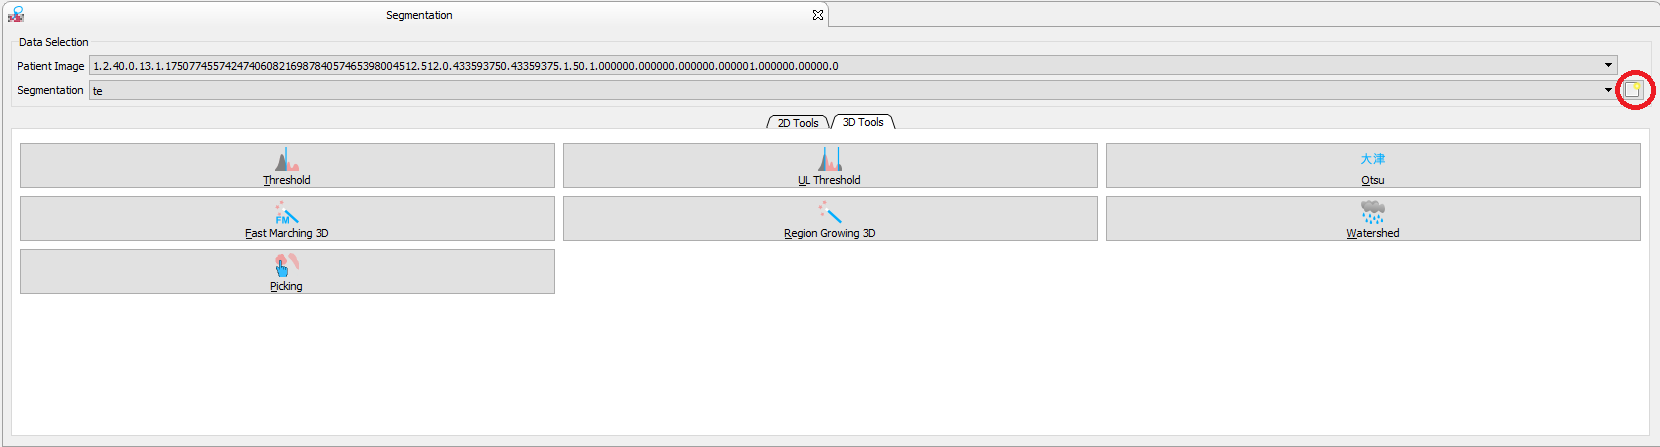
\includegraphics[width=0.7\textwidth]{Logos/MITK_Doku/6.PNG}
\caption{3D-Segmentierungstools  der MITK-Workbench} 
\label{fig:sechs} 
\end{figure}

Anschließend kann mit Shift + Linke Maustaste eine Punkt im Volumen ausgewählt werden. Danach muss mit  \textit{Run Segmentation} die Segmentierung ausgeführt werden.

\begin{figure}[H] 
\centering 
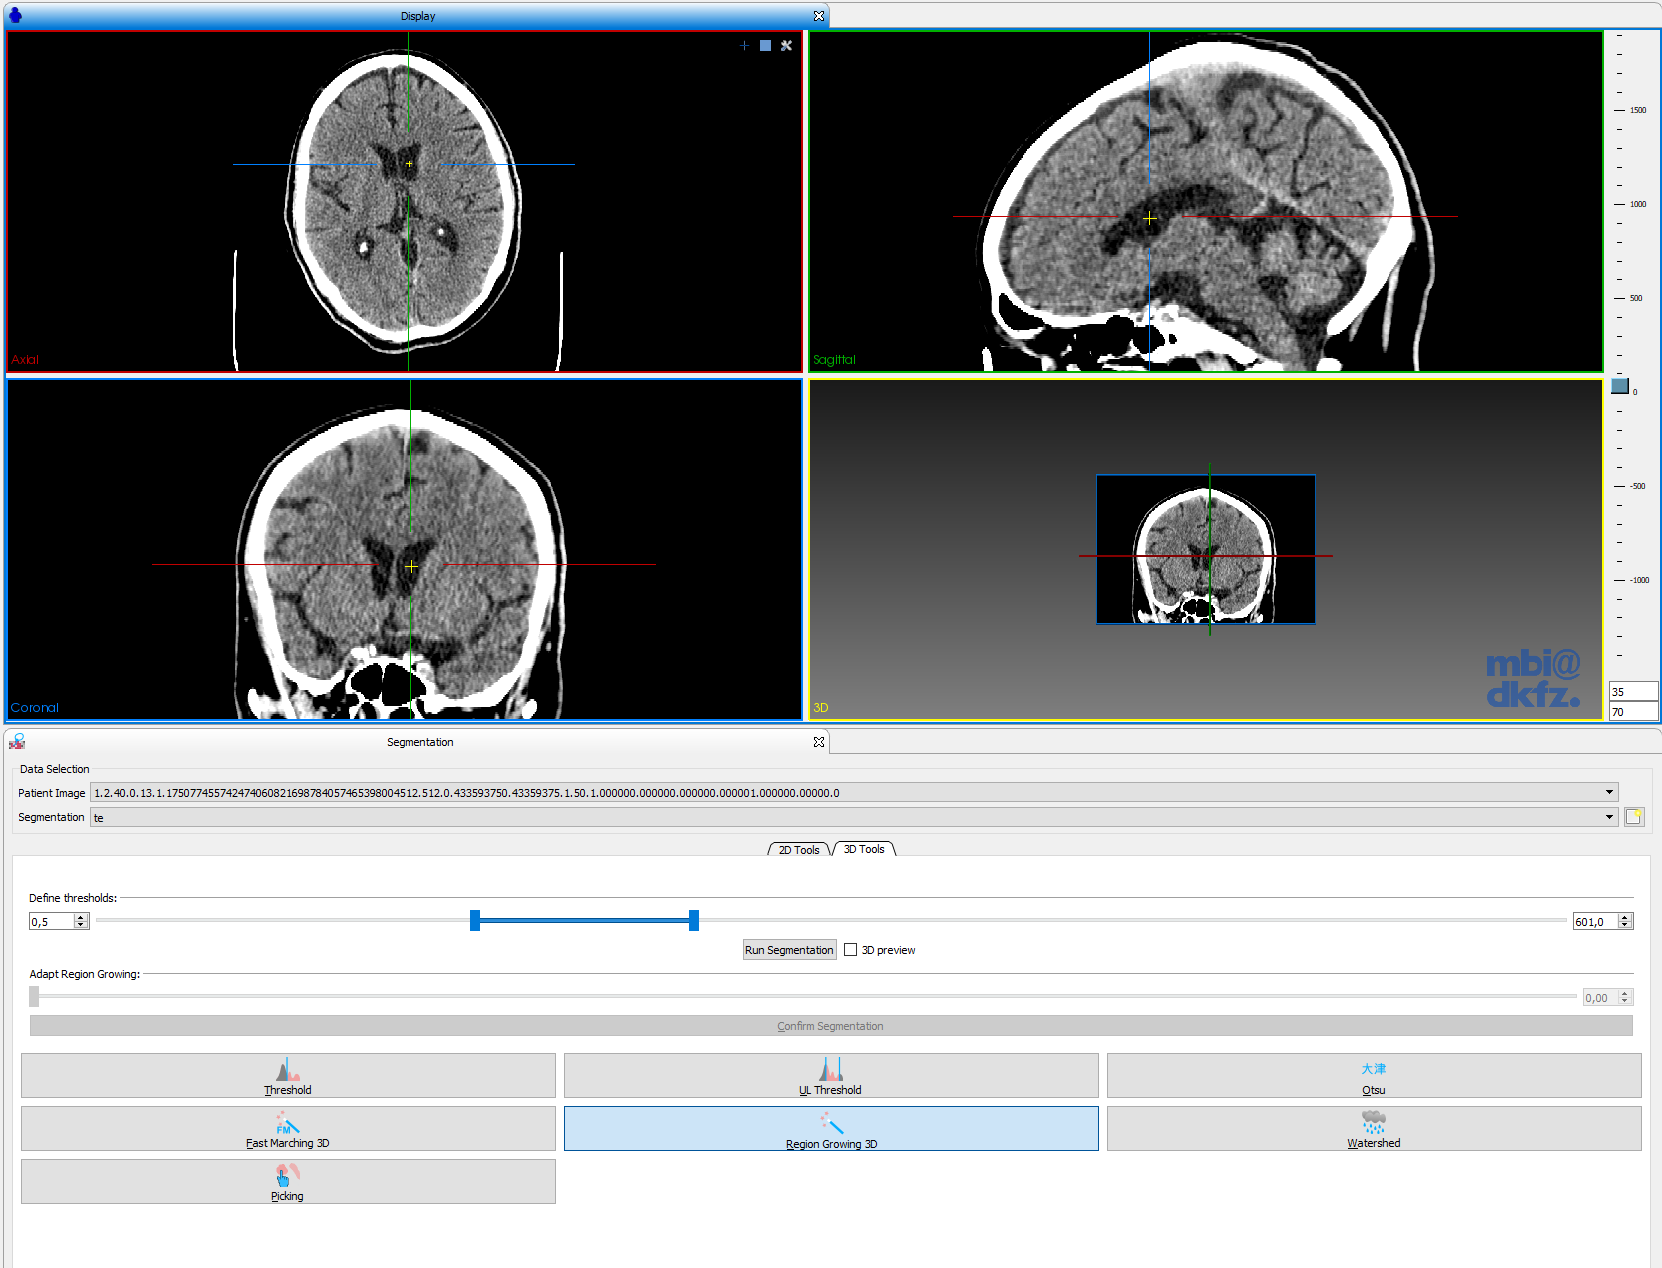
\includegraphics[width=0.7\textwidth]{Logos/MITK_Doku/7.PNG}
\caption{Region Growing Tool der MITK-Workbench} 
\label{fig:sieben} 
\end{figure}

Nun kann der Threshhold angepasst und das Region Growing mit dem \textit{Adapt Region Growing} Regler angepasst werden. Wird das gezielte Ergebnis erwünscht, kann es mit \textit{Confirm Segmentation} bestätigt werden.

\begin{figure}[H] 
\centering 
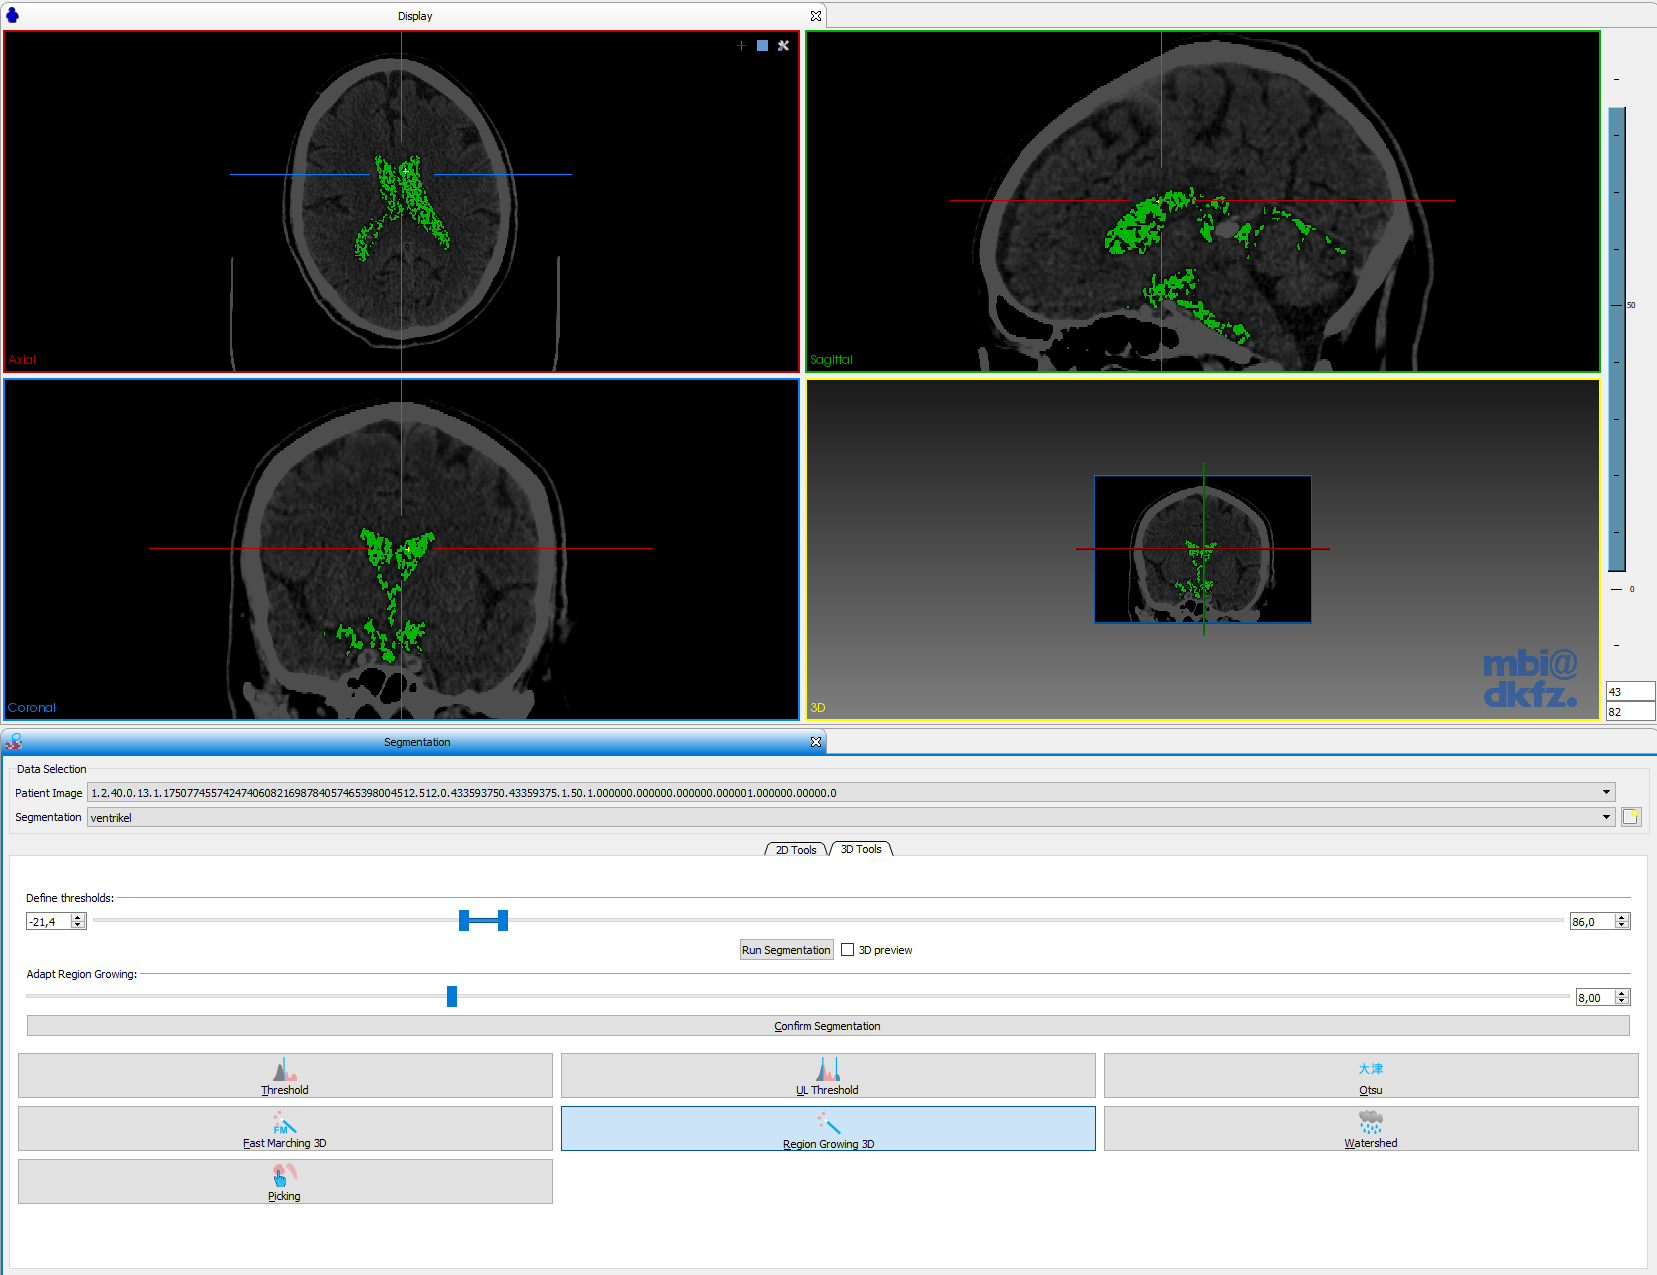
\includegraphics[width=0.7\textwidth]{Logos/MITK_Doku/8.PNG}
\caption{Anpassen der Parameter des Region Growing Tools  der MITK-Workbench} 
\label{fig:acht} 
\end{figure}

Mit Tool Nummer 4 kann das Ergebnis mit verschiedenen Operationen verbessert werden. Hierbei wird oft \textit{Closing} benutzt. Anschließend kann mit Rechtsklick auf die Segmentierung im \textit{Data Manager} der Befehl \textit{Create smoothed polygon model} ausgeführt werden

\begin{figure}[H] 
\centering 
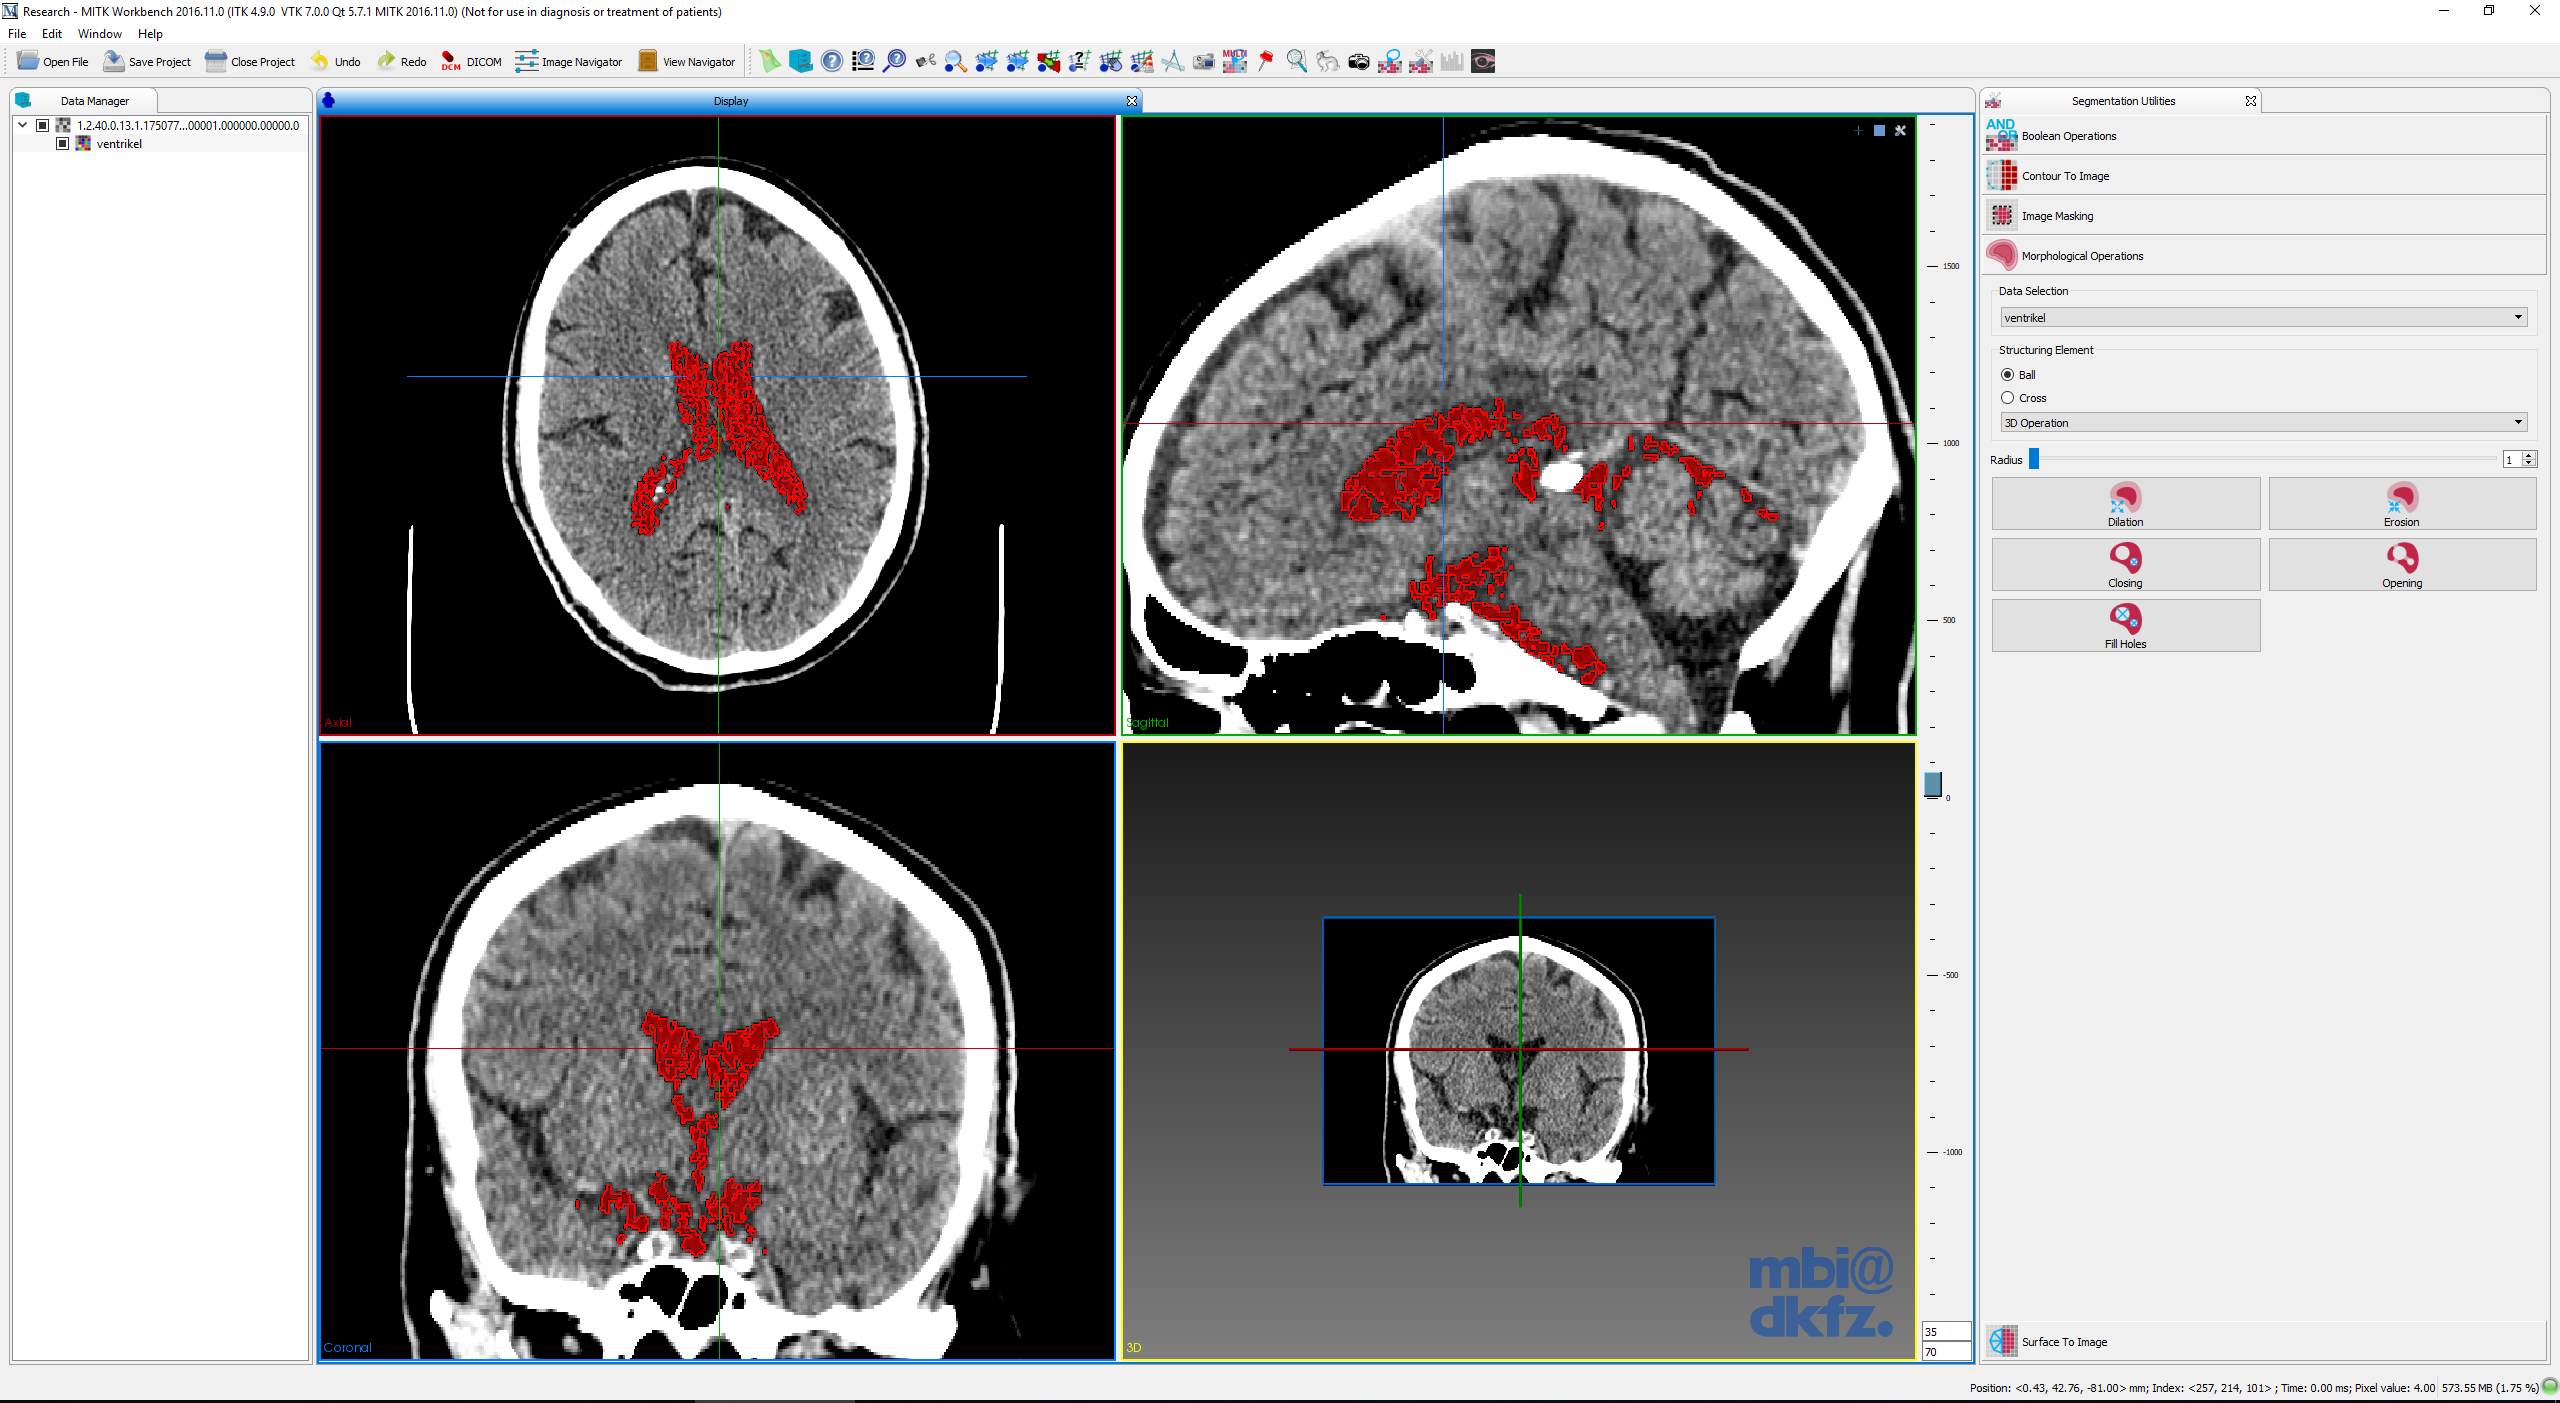
\includegraphics[width=0.7\textwidth]{Logos/MITK_Doku/9.PNG}
\caption{Filtertool der MITK-Workbench} 
\label{fig:neun} 
\end{figure}

Nachdem alle diese Schritte befolgt wurden ist im linken Unteren Kasten die Segmentierung sehen. Mit Tool Nummer 5 kann die Darstellung der Segmentierung verändert werden.

\begin{figure}[H] 
\centering 
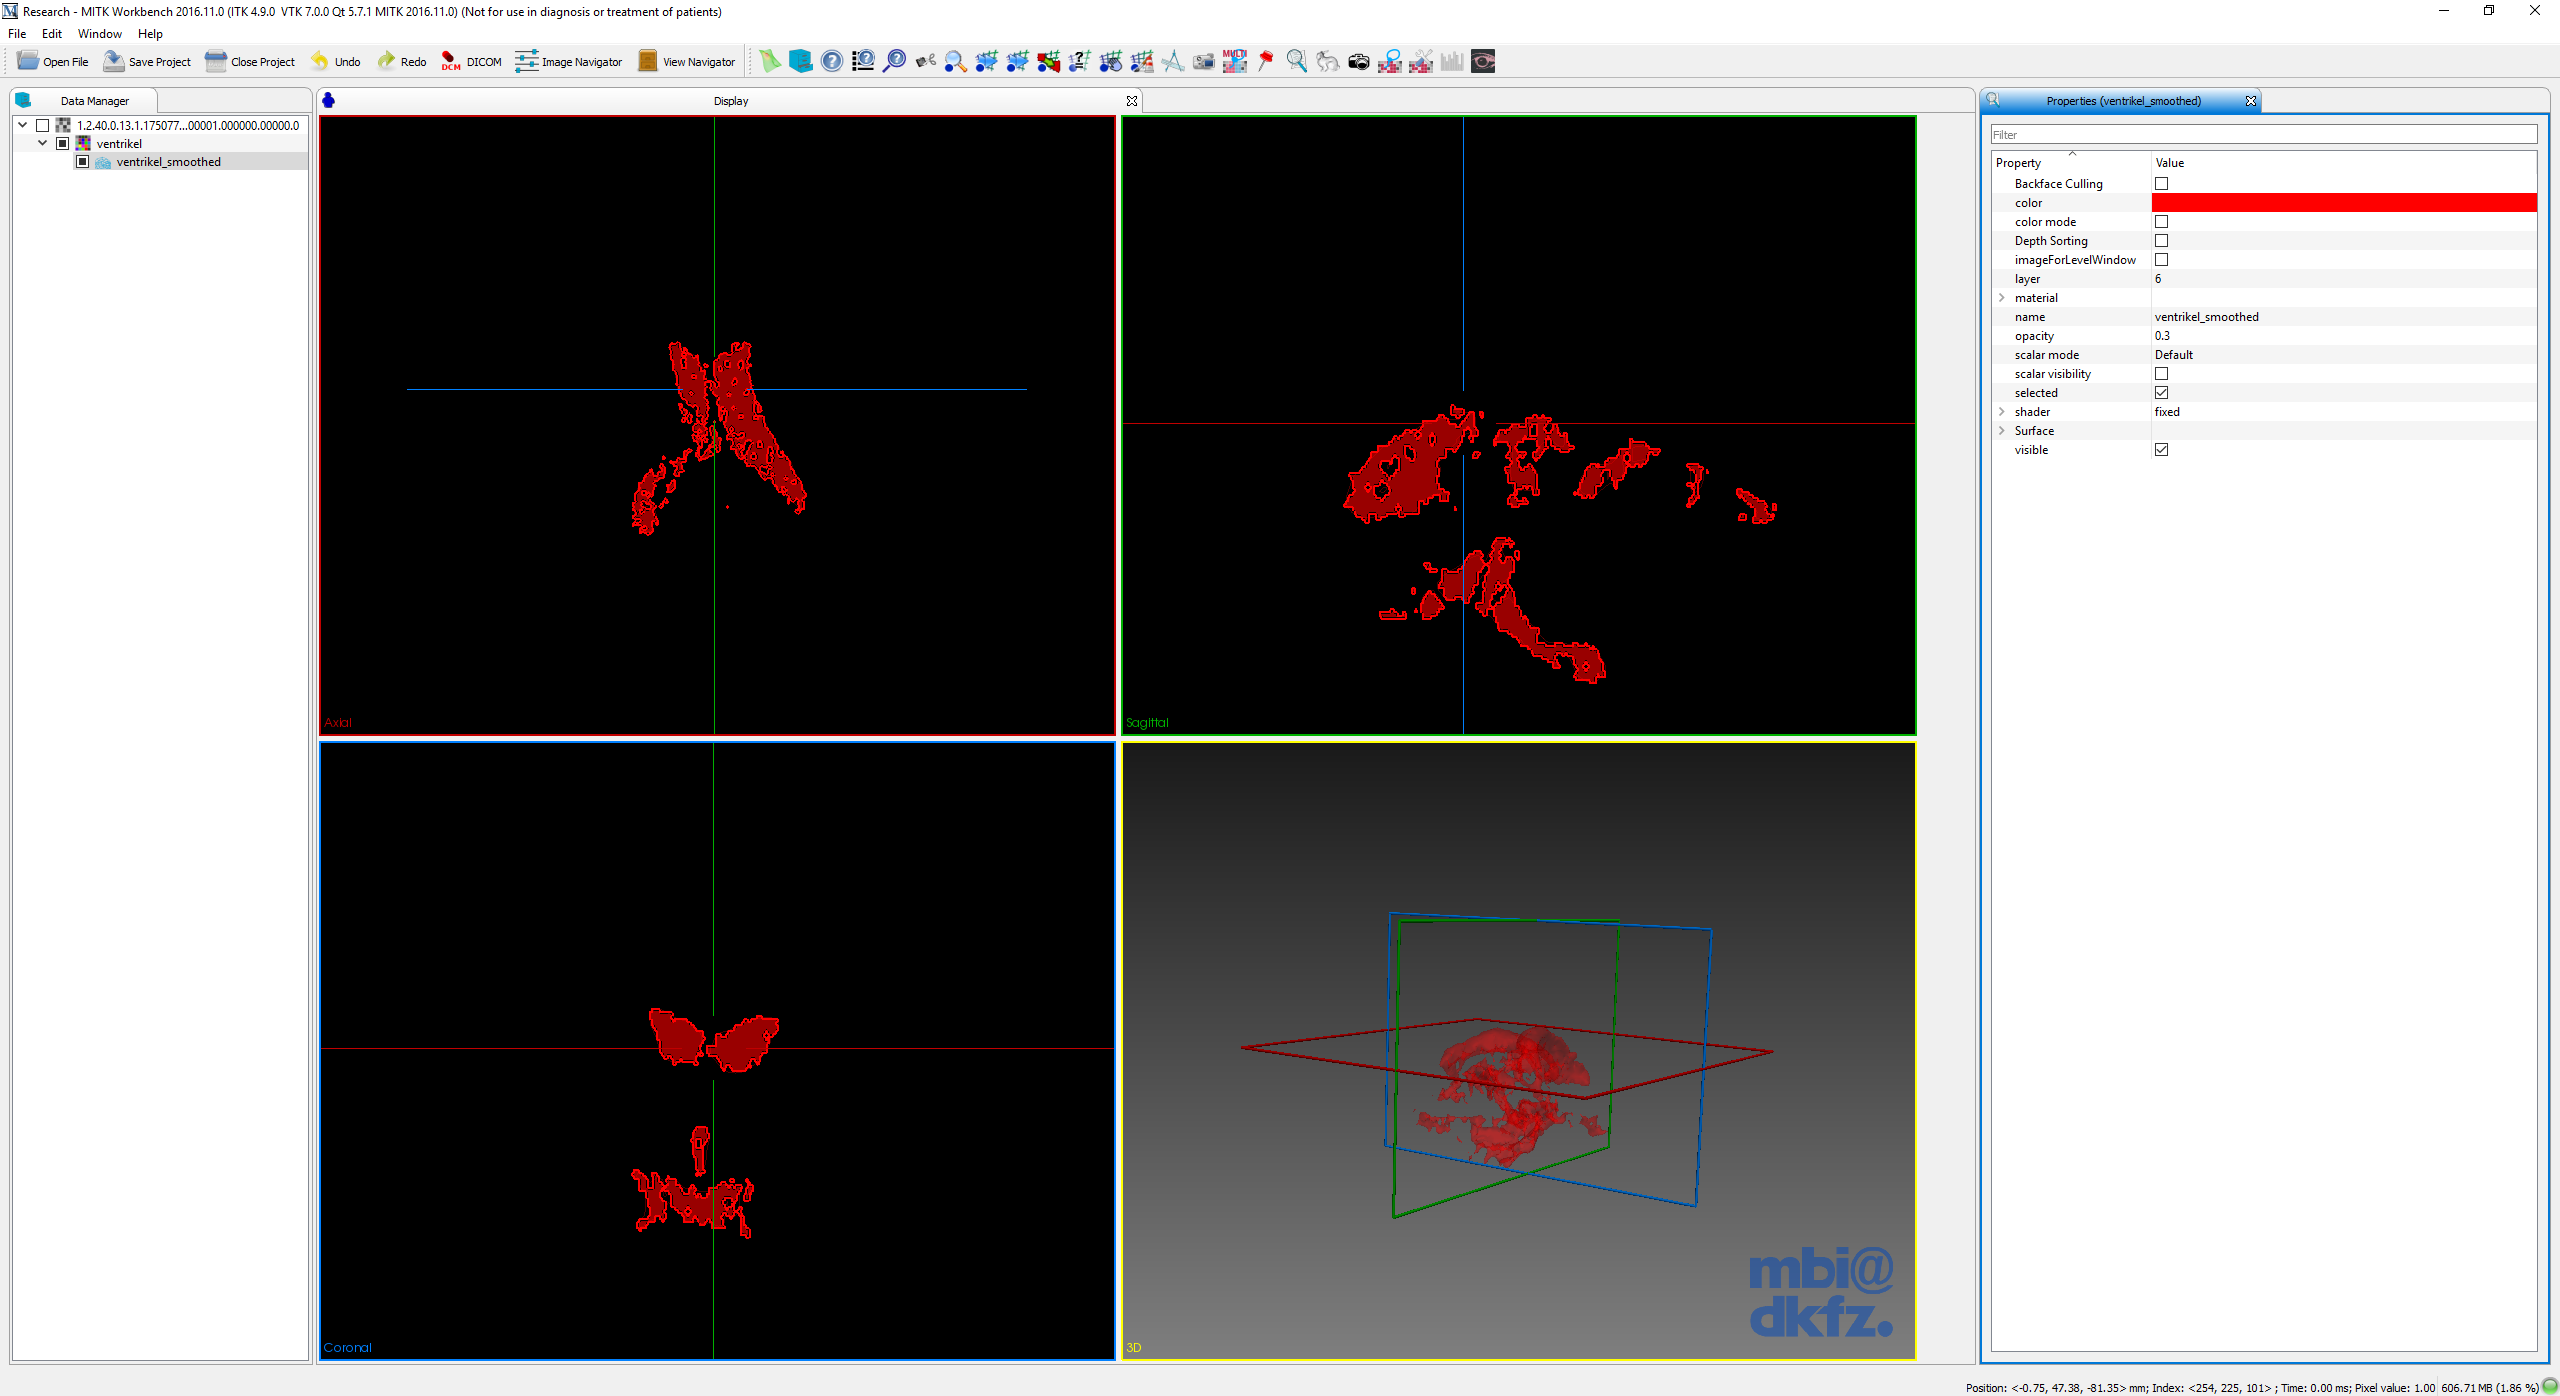
\includegraphics[width=0.7\textwidth]{Logos/MITK_Doku/10.PNG}
\caption{Darstellungstool der MITK-Workbench} 
\label{fig:zehn} 
\end{figure}